Prior to the derivation of the expected limits, we had to make sure their values are the most sensitive limits that our analysis can set. For that, we have done an optimization study finding the best cut value on the BDT discriminant with the idea to yield the lowest (the most sensitive) limit. For this study, before combination of electron and muon channels, we have optimized two channels separately. Systematical uncertainties were present only of the normalization type (lnN), since we are statistically limited and systematics plays a secondary role. %The latter can be seen running the fit with the "-S 0" option, which ignores systematics entirely. 
As an example, for a specific analysis setup the 300 GeV fit in the muon channel yields the limit ('r-value') 255.25 (with the systematics but neglecting BBB uncertainties), without systematics the 'r-value' is 238.25. The difference is 17 parts in 255.25, which is just 6.7 $\%$.

\subsection{Optimization for the best limit}

As can be seen from the plots ~\ref{fig:ele_bdt_vs_r} and ~\ref{fig:muon_bdt_vs_r}, for high mass region the best cut to use is 0.99 for both electron and muon channels. For low mass region, the situation is more complicated. Depending on the mass point (and channel!) one cut is better than the other. For electron channel for 400 and 450 GeV mass points the best cut is 0.925. In the lower region, the situation changes, 0.2 for 260 GeV, 0.4 for 270 and 300 GeV, 0.825 for 350 GeV. 

Running the whole analysis for each separate cut and channel and spin hypothesis is not possible computationally taking into account the number of samples and shapes one has to create and process. That is why a reasonable compromise is to observe that for 260 $\to$ 350 GeV included, the suboptimal cut can be 0.4, being well inside the $1\sigma$ error band. This leaves the whole mass range with just three different cut values. This approach of suboptimal cuts, cuts which are close the best values but, most importantly, can be shared among several mass points, is what we adopted for this measurement. 

For instance, for muons the best cuts are: 0.1 for 260 and 270 GeV, 0.5 for 300 GeV, 0.7 for 350 GeV, 0.925 for 400 and 450 GeV. Taking the approach of suboptimal cuts, the values we kept are: 0.1 for 260 and 270 GeV, 0.7 for 300 $\to$ 450 GeV included. This way we simplify the analysis to three different BDT cuts per channel and, at the same time, remain optimal within the error bands with respect to the best cut values. This is summarized in the Table~\ref{suboptCut}.

\begin{table}
\begin{center} 
  \caption{Suboptimal BDT cuts used in the analysis}
 \begin{tabular}{ |c|c|c|c|c| } \hline%\hline
   channel & 260 and 270 GeV & 300 and 350 GeV & 400 and 450 GeV & 600 GeV to 1000 GeV \\ \hline
   muons & 0.1 & 0.7 & 0.7 & 0.99 \\ %\hline
   electrons & 0.4 & 0.4 & 0.925 & 0.99\\ \hline%\hline
  \end{tabular}
  \label{suboptCut}
\end{center}   
\end{table}









\begin{figure}[!htb]%hbpt?        
\includegraphics[width=0.5\textwidth, height=0.2\textheight,  keepaspectratio]{eles_bdt_vs_r/gr_limits__260GeV.pdf}
\includegraphics[width=0.5\textwidth, height=0.2\textheight,  keepaspectratio]{eles_bdt_vs_r/gr_limits__270GeV.pdf}
\includegraphics[width=0.5\textwidth, height=0.2\textheight,  keepaspectratio]{eles_bdt_vs_r/gr_limits__300GeV.pdf}
\includegraphics[width=0.5\textwidth, height=0.2\textheight,  keepaspectratio]{eles_bdt_vs_r/gr_limits__350GeV.pdf}
\includegraphics[width=0.5\textwidth, height=0.2\textheight,  keepaspectratio]{eles_bdt_vs_r/gr_limits__400GeV.pdf}
\includegraphics[width=0.5\textwidth, height=0.2\textheight, keepaspectratio]{eles_bdt_vs_r/gr_limits__450GeV.pdf}
\includegraphics[width=0.5\textwidth, height=0.2\textheight, keepaspectratio]{eles_bdt_vs_r/gr_limits__600GeV.pdf}
\includegraphics[width=0.5\textwidth, height=0.2\textheight, keepaspectratio]{eles_bdt_vs_r/gr_limits__650GeV.pdf}
\includegraphics[width=0.5\textwidth, height=0.2\textheight, keepaspectratio]{eles_bdt_vs_r/gr_limits__900GeV.pdf}
\hspace{1.9cm}
\includegraphics[width=0.5\textwidth, height=0.2\textheight, keepaspectratio]{eles_bdt_vs_r/gr_limits__1000GeV.pdf}
\caption{ Cut on the BDT output vs 'r-value' from Combine. Electron channel.}
\label{fig:ele_bdt_vs_r}                                                       
\end{figure}



\begin{figure}[!htb]%hbpt?        
\includegraphics[width=0.5\textwidth, height=0.2\textheight, keepaspectratio]{muons_bdt_vs_r/gr_limits__260GeV.pdf}
\includegraphics[width=0.5\textwidth, height=0.2\textheight, keepaspectratio]{muons_bdt_vs_r/gr_limits__270GeV.pdf}
\includegraphics[width=0.5\textwidth, height=0.2\textheight, keepaspectratio]{muons_bdt_vs_r/gr_limits__300GeV.pdf}
\includegraphics[width=0.5\textwidth, height=0.2\textheight, keepaspectratio]{muons_bdt_vs_r/gr_limits__350GeV.pdf}
\includegraphics[width=0.5\textwidth, height=0.2\textheight, keepaspectratio]{muons_bdt_vs_r/gr_limits__400GeV.pdf}
\includegraphics[width=0.5\textwidth, height=0.2\textheight, keepaspectratio]{muons_bdt_vs_r/gr_limits__450GeV.pdf}
\includegraphics[width=0.5\textwidth, height=0.2\textheight, keepaspectratio]{muons_bdt_vs_r/gr_limits__600GeV.pdf}
\includegraphics[width=0.5\textwidth, height=0.2\textheight, keepaspectratio]{muons_bdt_vs_r/gr_limits__650GeV.pdf}
\includegraphics[width=0.5\textwidth, height=0.2\textheight, keepaspectratio]{muons_bdt_vs_r/gr_limits__900GeV.pdf}
\hspace{1.9cm}
\includegraphics[width=0.5\textwidth, height=0.2\textheight, keepaspectratio]{muons_bdt_vs_r/gr_limits__1000GeV.pdf}
\caption{ Cut on the BDT output vs 'r-value' from Combine. Muon channel.}
\label{fig:muon_bdt_vs_r}           
\end{figure}

 
\subsection{Results from the fit}
The extraction of the results is performed by what is called at CMS "Binned shape analysis". We used Higgs Combination Tool ("HiggsCombine")~\cite{HiggsCombine}, which is a framework with the help of which the Higgs boson has been discovered. HiggsCombine is based on the RooStats package that has been very popular in the HEP community for years. 

We do a simultaneous fit (\mTHH transverse mass distribution is used) of all three
regions: signal region and two control regions, to extract both
signal strength parameter as well as normalizations of \ttbar and
Drell-Yan backgrounds. We use the following command to produce expected limits with the Asimov ~\cite{Cowan:2010js} toy dataset :  \hfill \break
$\textit{combine 
-M Asymptotic -t -1 -v 3 -m massValue --run blind
comb\_card\_massValue.txt}$.





The results in the Table ~\ref{finalLimits} are final limits produced with the combined data of electron and muon channels. The corresponding plots, from which these number were extracted, are shown on the Figs. ~\ref{fig:HHlimits}. %Separately limits for electron and muon channels are shown at the Figs. ~\ref{fig:HHlimits}. 

%The values of the DY and \ttbar normalizations in control regions extracted during the simultaneous fit of signal and control regions are shown in the Tables ~\ref{normalization_electron}, ~\ref{normalization_muon}.%, and ~\ref{normalization_comb}. 
Full postfit distributions (the naming emphasises that all regions are used in the fit, signal region included) are shown on the Figs. ~\ref{fig:MCcomparisons} for the graviton case and ~\ref{fig:MCcomparisons_radion} for the radion case. 
%Comprehensive study with per channel distributions and for different mass regions can be found on Figs. ~\ref{fig:MCcomparison_mm_300} - ~\ref{fig:MCcomparison_ee_900}.

%The corresponding values of the DY and \ttbar normalizations in the unblinded SR control regions are shown in the Tables ~\ref{normalization_electron_SR}, ~\ref{normalization_muon_SR}.






\begin{figure}[!htb]%hbpt?                                                                                        
  \begin{center}
%    \raisebox{0.17\height}                                                                                       
    %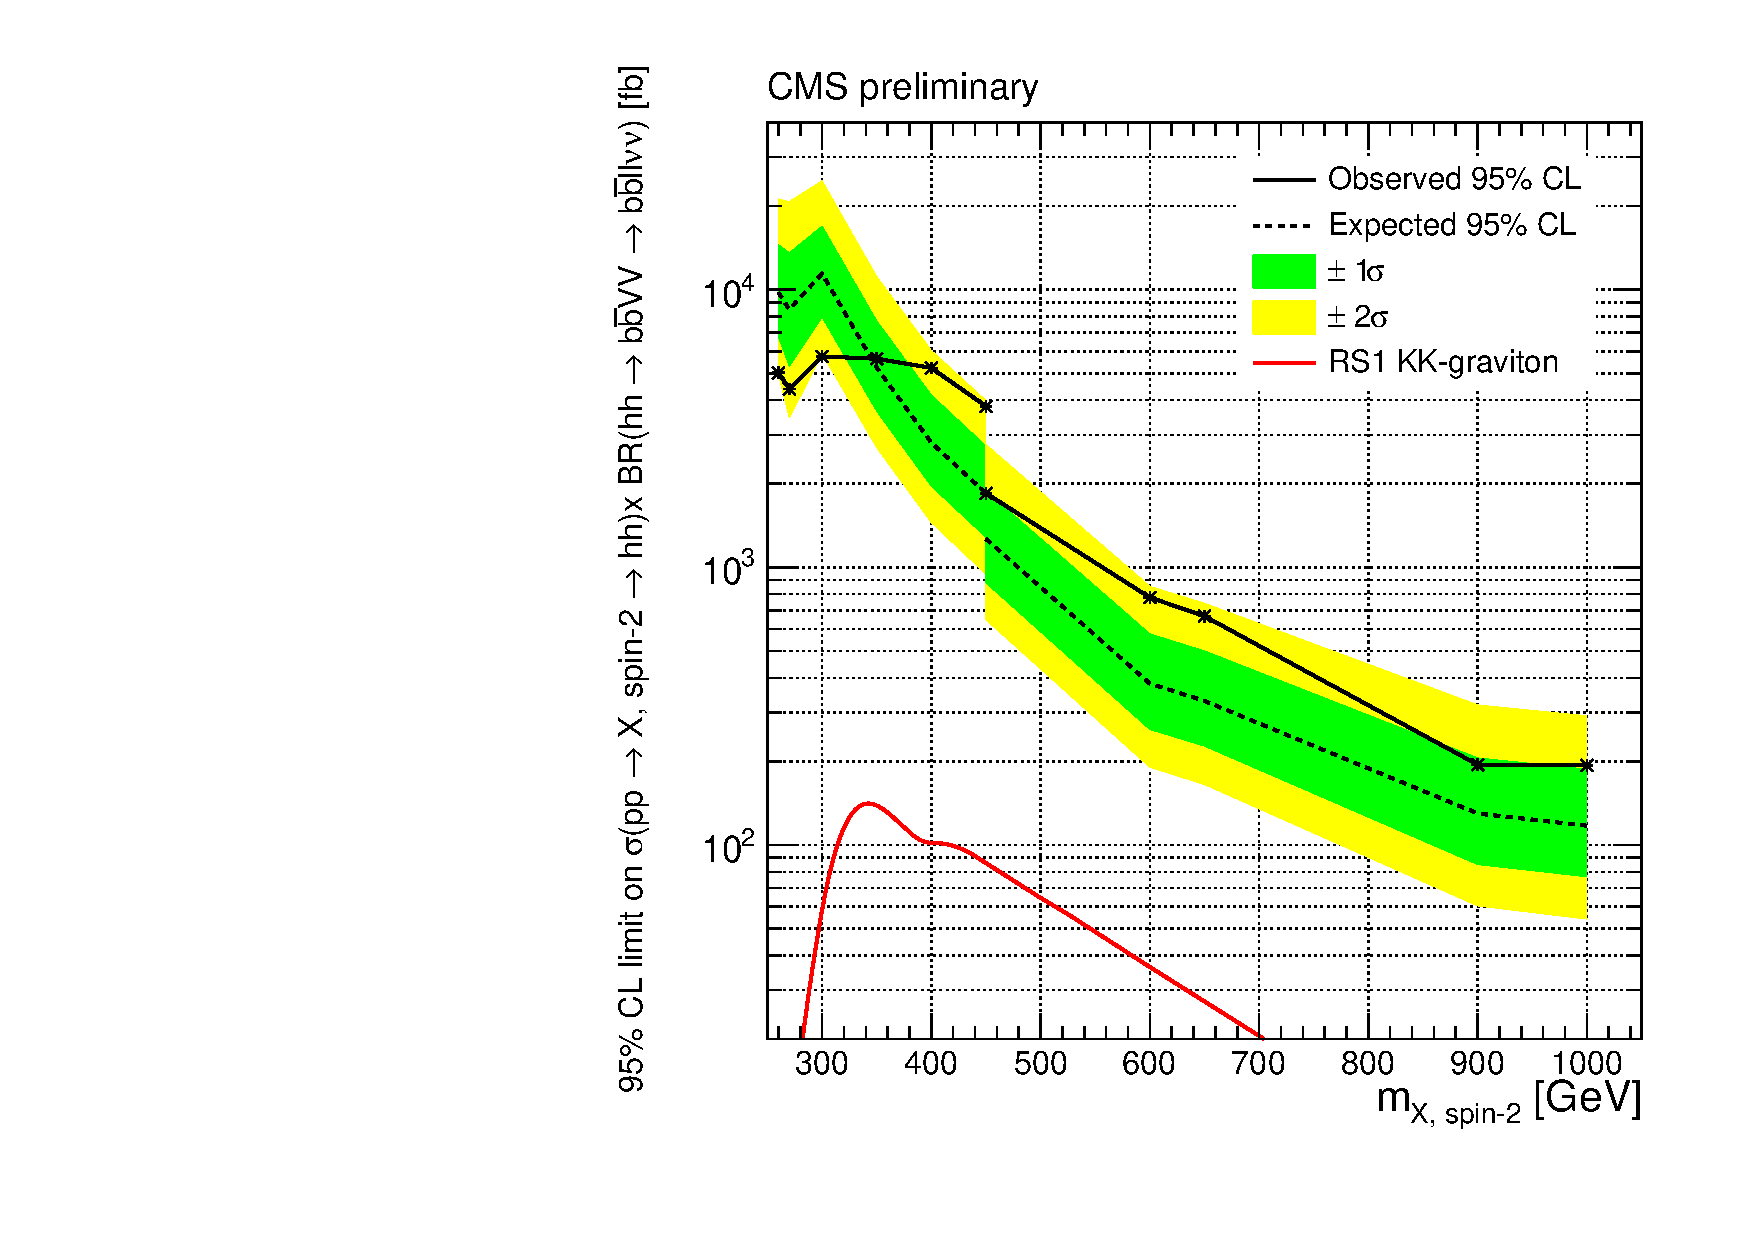
\includegraphics[width=0.65\textwidth]{limitbbZZ_apr29_comb.pdf}                                     
    %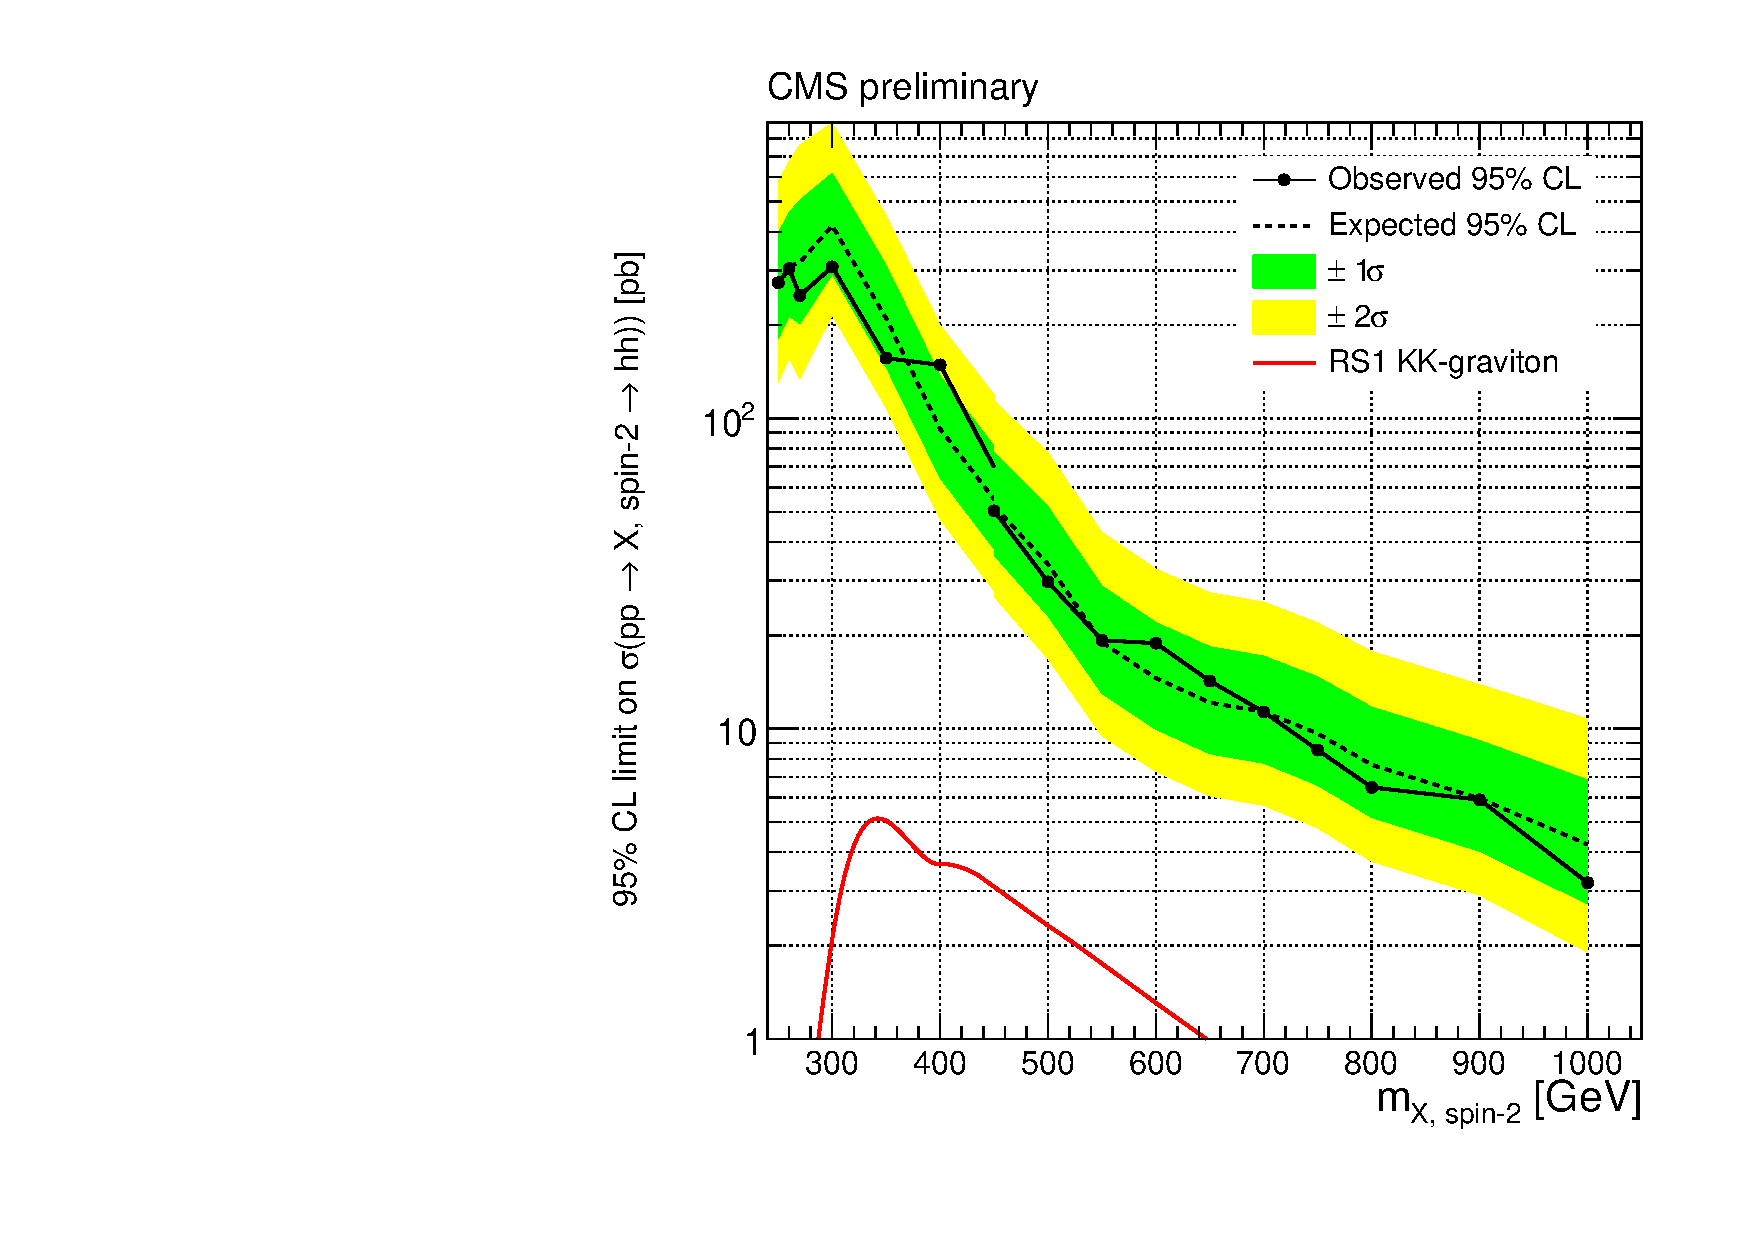
\includegraphics[width=0.65\textwidth]{limitHH_June13_comb.pdf}                                      
    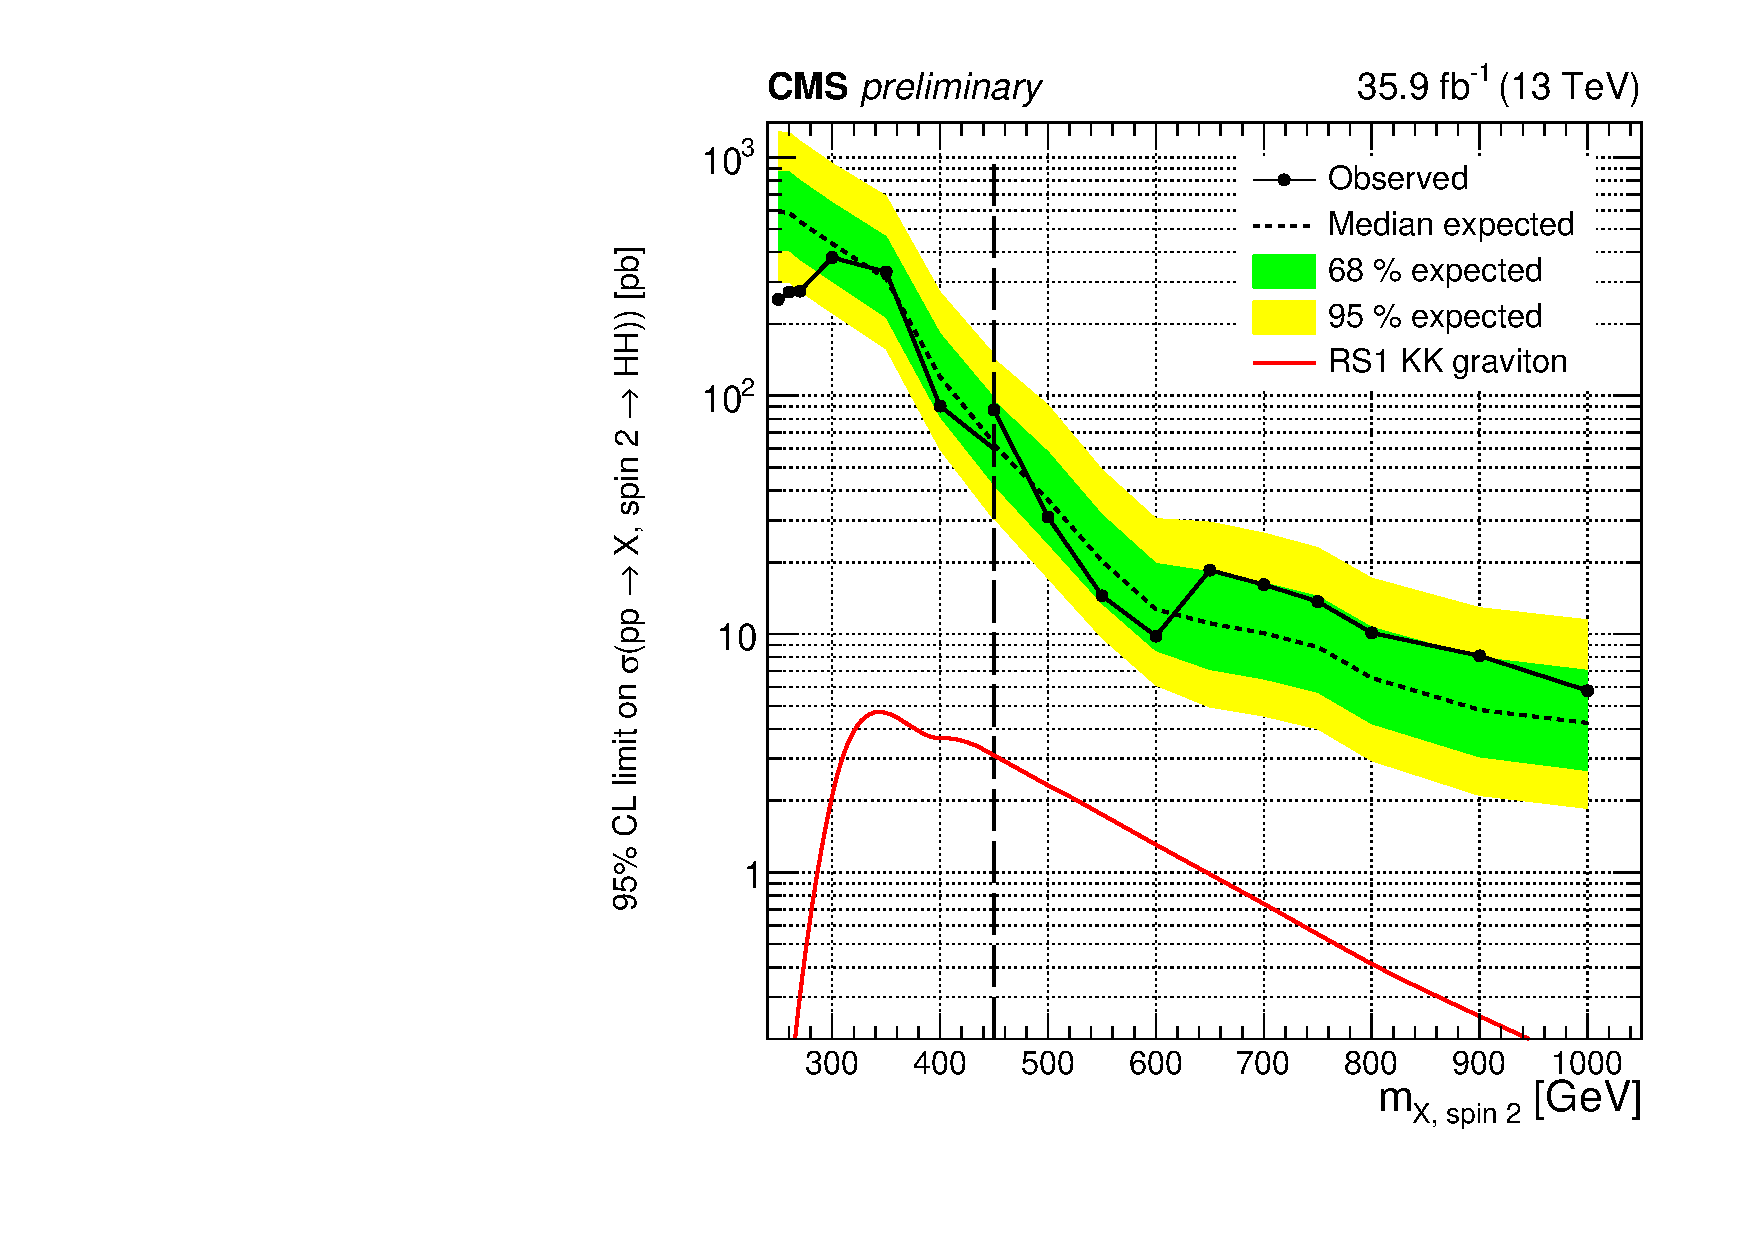
\includegraphics[width=0.65\textwidth]{limitHH_Nov16_graviton.pdf}
    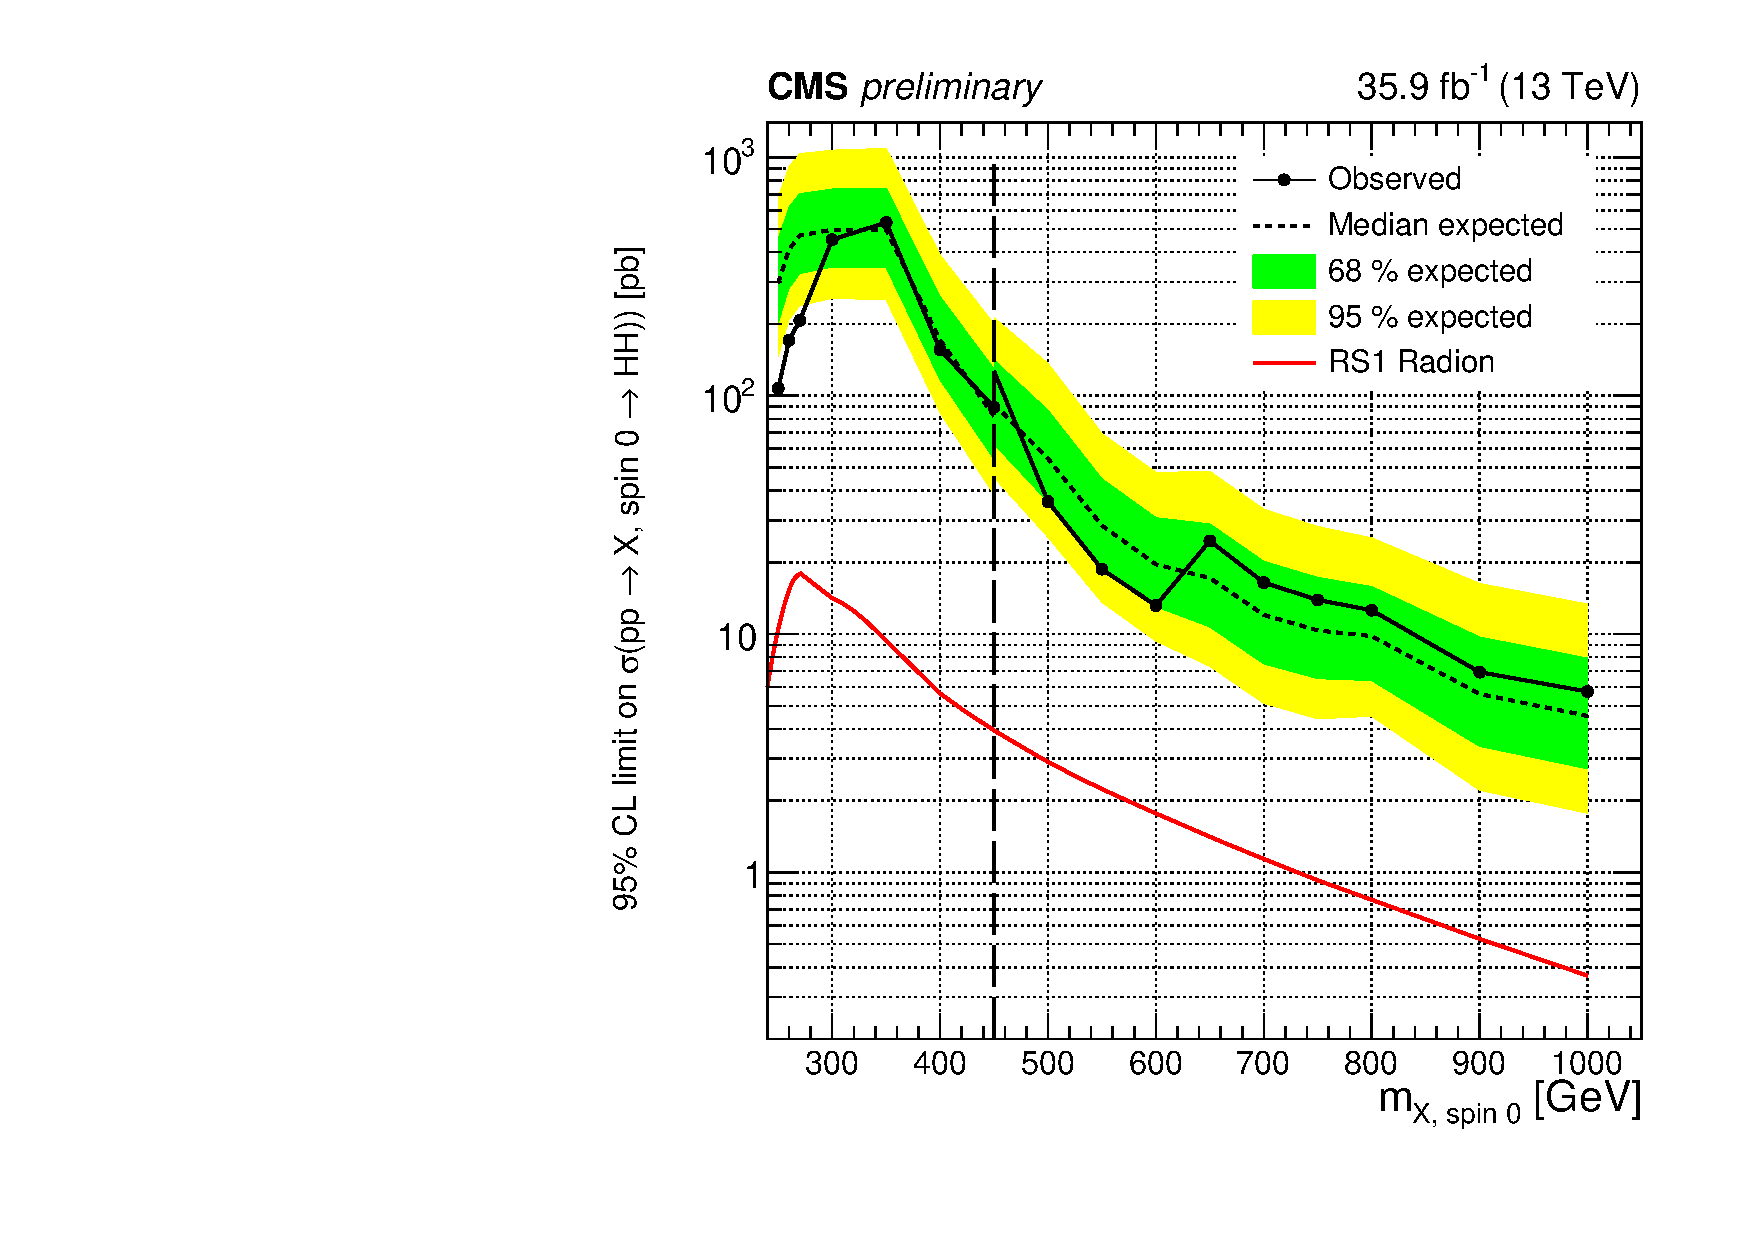
\includegraphics[width=0.65\textwidth]{limitHH_Nov16_radion.pdf}
    \caption{ Expected (dashed line) and observed (solid line) limits on the cross section of a resonant HH production
      as a function of the mass of the narrow resonance for both leptonic channels combined. Graviton case is shown at the top and radion case at the bottom. The red line shows a theoretical prediction for
      the production of a WED particle with certain model assumptions \cite{Oliveira:2014kla}.
      }
      % Expected and observed limits on the HH production.                                                        
     %Top: in the 2 b jets, 2 lepton, 2 neutrinos final state optimized for the bbZZ selection. Bottom: full HH production.                                                                                                        
    \label{fig:HHlimits} %bbZZlimits                                                                              
  \end{center}
\end{figure}




%sept28
\begin{table}
\begin{center}
\caption{The expected and observed HH production cross section upper limits at 95\% CL for different
narrow resonance graviton (top) and radion (bottom) mass hypotheses for both dielectron and dimuon channels combined.}
\label{finalLimits}
\begin{tabular}{|c|c|c|}
%\toprule                                                                                                                                        
\hline
Mass, GeV &  Observed Limit, pb &  Expected Limit, pb \\
\hline
%\midrule                                                                                                                                        
      250 &               253.5 &               589.1 \\
      260 &               272.2 &               585.9 \\
      270 &               274.4 &               537.5 \\
      300 &               380.0 &               434.4 \\
      350 &               330.6 &               309.4 \\
      400 &                90.4 &               119.9 \\
      450 &                59.8 &                63.3 \\
      500 &                31.0 &                36.6 \\
      550 &                14.5 &                20.2 \\
      600 &                 9.8 &                12.7 \\
      650 &                18.5 &                11.1 \\
      700 &                16.1 &                10.1 \\
      750 &                13.7 &                 8.8 \\
      800 &                10.1 &                 6.5 \\
      900 &                 8.1 &                 4.8 \\
     1000 &                 5.8 &                 4.2 \\
%\bottomrule                                                                                                                                     
\hline
\end{tabular}
%% \end{center}                                                                                                                                  
%% \end{table}                                                                                                                                   
%% \begin{table}                                                                                                                                 
%% \begin{center}                                                                                                                                
%\caption{The expected and observed HH production cross section upper limits at 95\% CL for different narrow resonance Radion mass hypotheses for both dielectron and dimuon channels combined.}                                                                                                 
\vspace{1 cm} \ \\
%\label{tab:finalLimits}                                                                                                                         
\begin{tabular}{|c|c|c|}
%\toprule                                                                                                                                        
\hline
Mass, GeV &  Observed Limit, pb &  Expected Limit, pb \\
\hline
%\midrule                                                                                                                                        
     250 &               107.3 &               297.7 \\
     260 &               170.8 &               410.9 \\
     270 &               207.0 &               470.3 \\
     300 &               451.7 &               496.9 \\
     350 &               532.6 &               496.9 \\
     400 &               155.7 &               171.1 \\
     450 &                89.3 &                82.0 \\
     500 &                36.0 &                54.4 \\
     550 &                18.7 &                28.5 \\
     600 &                13.2 &                19.6 \\
     650 &                24.6 &                17.2 \\
     700 &                16.4 &                12.0 \\
     750 &                13.9 &                10.4 \\
     800 &                12.6 &                 9.8 \\
     900 &                 6.9 &                 5.6 \\
    1000 &                 5.7 &                 4.5 \\
%\bottomrule                                                                                                                                     
\hline
\end{tabular}
\end{center}
\end{table}


%For the HL-LHC none of the HH analyses can reach the discovery sensitivity, thus the goal for all HH analyses is to contribute to the grand combination and in this collaborative way to achieve the desired sensitivity. The most recent combination results for the spin 0 case are shown at the Fig. \ref{HH_combo}.



%% \begin{figure}[!htb]%hbpt?                                                                                                               
%% 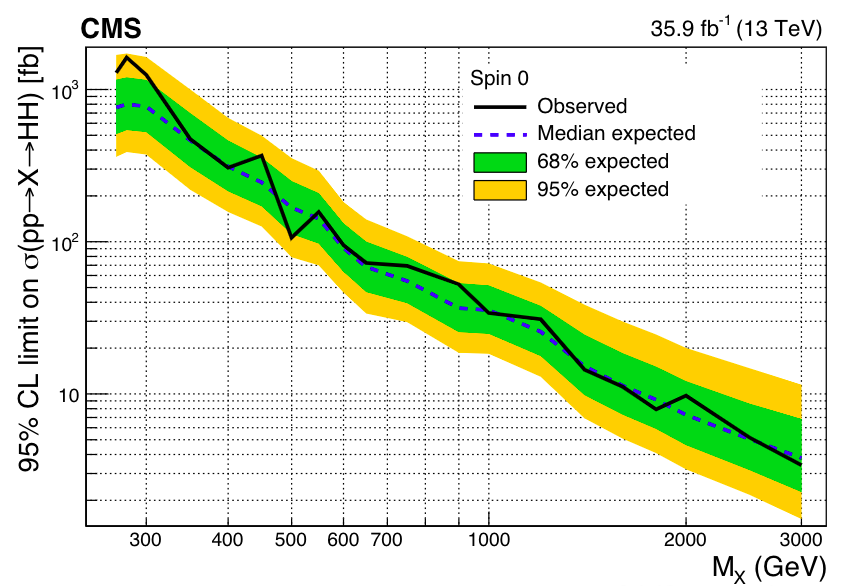
\includegraphics[width=0.5\textwidth, height=0.2\textheight,  keepaspectratio]{spin0_combo.png}
%% \caption{ The current combination of HH channels for the spin 0 heavy resonance hypothesis. }
%% \label{HH_combo}
%% \end{figure}









%% %added on dec17
%% \begin{table}
%% \begin{center}
%% \caption{Expected limits for full HH production. Combined data is used.}
%% \label{finalLimits}
%% \begin{tabular}{|c|c|}
%% \hline
%%  Mass, GeV &  Expected limit, pb \\\hline
%%       260 &              274.00 \\
%%        270 &              306.50 \\
%%        300 &              306.00 \\
%%        350 &              141.88 \\
%%        400 &               59.00 \\
%%        450 &               34.12 \\
%%        600 &                7.69 \\
%%        650 &                6.31 \\
%%        900 &                2.59 \\
%%       1000 &                2.25 \\\hline

%% \end{tabular}
%% \end{center}
%% \end{table}









%
%
%%Vertical lines as column separators
%\begin{table}
%\begin{center}
%\caption{Normalization for backgrounds, final numbers after the application of all the nuisances during the postfit procedure. Electron channel.}
%\begin{tabular}{ | c | c | c | }
%  \hline
%  channel,mass & TT\_SF & DY\_SF \\
%  \hline
%  ee 300 GeV    & 0.80 +/- 0.09   &  1.62 +/- 0.23\\
%  ee 900 GeV    & 0.79 +/- 0.08    & 1.64 +/- 0.18\\
%  \hline
%\end{tabular}
%\label{normalization_electron}
%\end{center}
%%---------------------------------------------------------------------
%%Vertical lines as column separators
%\begin{center}
%\caption{Normalisation for backgrounds in the unblinded SR, final numbers after the application of all the nuisances during the postfit procedure. Electron channel.}
%\begin{tabular}{ | c | c | c | }
%  \hline
%  channel,mass & TT\_SF & DY\_SF \\
%  \hline
%  ee 300 GeV    &  0.8 +/- 0.1    &   1.58 +/- 0.25 \\
%%fit_s
% ee 900 GeV    &  0.9 +/- 0.33     &  1.75 +/- 0.49\\
%%from  log_PostFitShapesFromWorkspace_ee_SR_hhMt_FullPostfit.txt
%  \hline
%\end{tabular}
%\label{normalization_electron_SR}
%\end{center}
%\end{table}
%%---------------------------------------------------------------------
%
%
%%\vspace{1cm}
%\begin{table}
%\begin{center}
%\caption{Normalization for backgrounds, final numbers after the application of all the nuisances during the postfit procedure. Muon channel.}
%\begin{tabular}{ | c | c | c | }
%  \hline
%  channel,mass & TT\_SF & DY\_SF \\
%  \hline
%  mm 300 GeV   & 0.91 +/- 0.07 & 1.44 +/- 0.13\\
%  mm 900 GeV   & 0.91 +/- 0.07 & 1.43 +/- 0.13\\
%
%  \hline
%\end{tabular}
%\label{normalization_muon}
%\end{center}
%%\vspace{1cm}
%\begin{center}
%\caption{Normalisation for backgrounds in the unblinded SR, final numbers after the application of all the nuisances during the postfit procedure. Muon channel.}
%
%\begin{tabular}{ | c | c | c | }
%  \hline
%  channel,mass & TT\_SF & DY\_SF \\
%  \hline
%  mm 300 GeV   &  0.91 +/- 0.07  & 1.49 +/- 0.15\\
%  mm 900 GeV   &  0.91 +/- 0.19  & 1.53 +/- 0.42\\
%
%  \hline
%\end{tabular}
%\label{normalization_muon_SR}
%\end{center}
%\end{table}


